\subsection{Modelo de negocios en un videojuego}\label{modeloNegocio}
Para sustentar un proyecto o producto económicamente se debe tener claro un modelo de negocios. En el mundo de los videojuegos no existe la excepción, pero también debe considerarse que existen formas muy diferentes de adquirir el ingreso.

Incluso el mismo juego puede estar involucrado en un ingreso directo del servicio.

\subsubsection{Mercado global}
Se reporta segun Newzoo \cite{newzoo2018} que 2.3 billones de jugadores en todo el mundo gastarán \$ 137.9 billones en juegos en 2018. Esto representa un aumento de + 13.3\% en comparación con el año anterior, o \$ 16.2 billones. Los ingresos por juegos digitales tomarán el 91\% del mercado global con \$ 125.3 mil millones, como podemos ver en la \ref{fig:merglo}
\begin{figure}
	\centering
	\caption{Mércado global al primer trimestre del año 2018 por Newzoo \cite{newzoo2018}}
	\label{fig:merglo}
	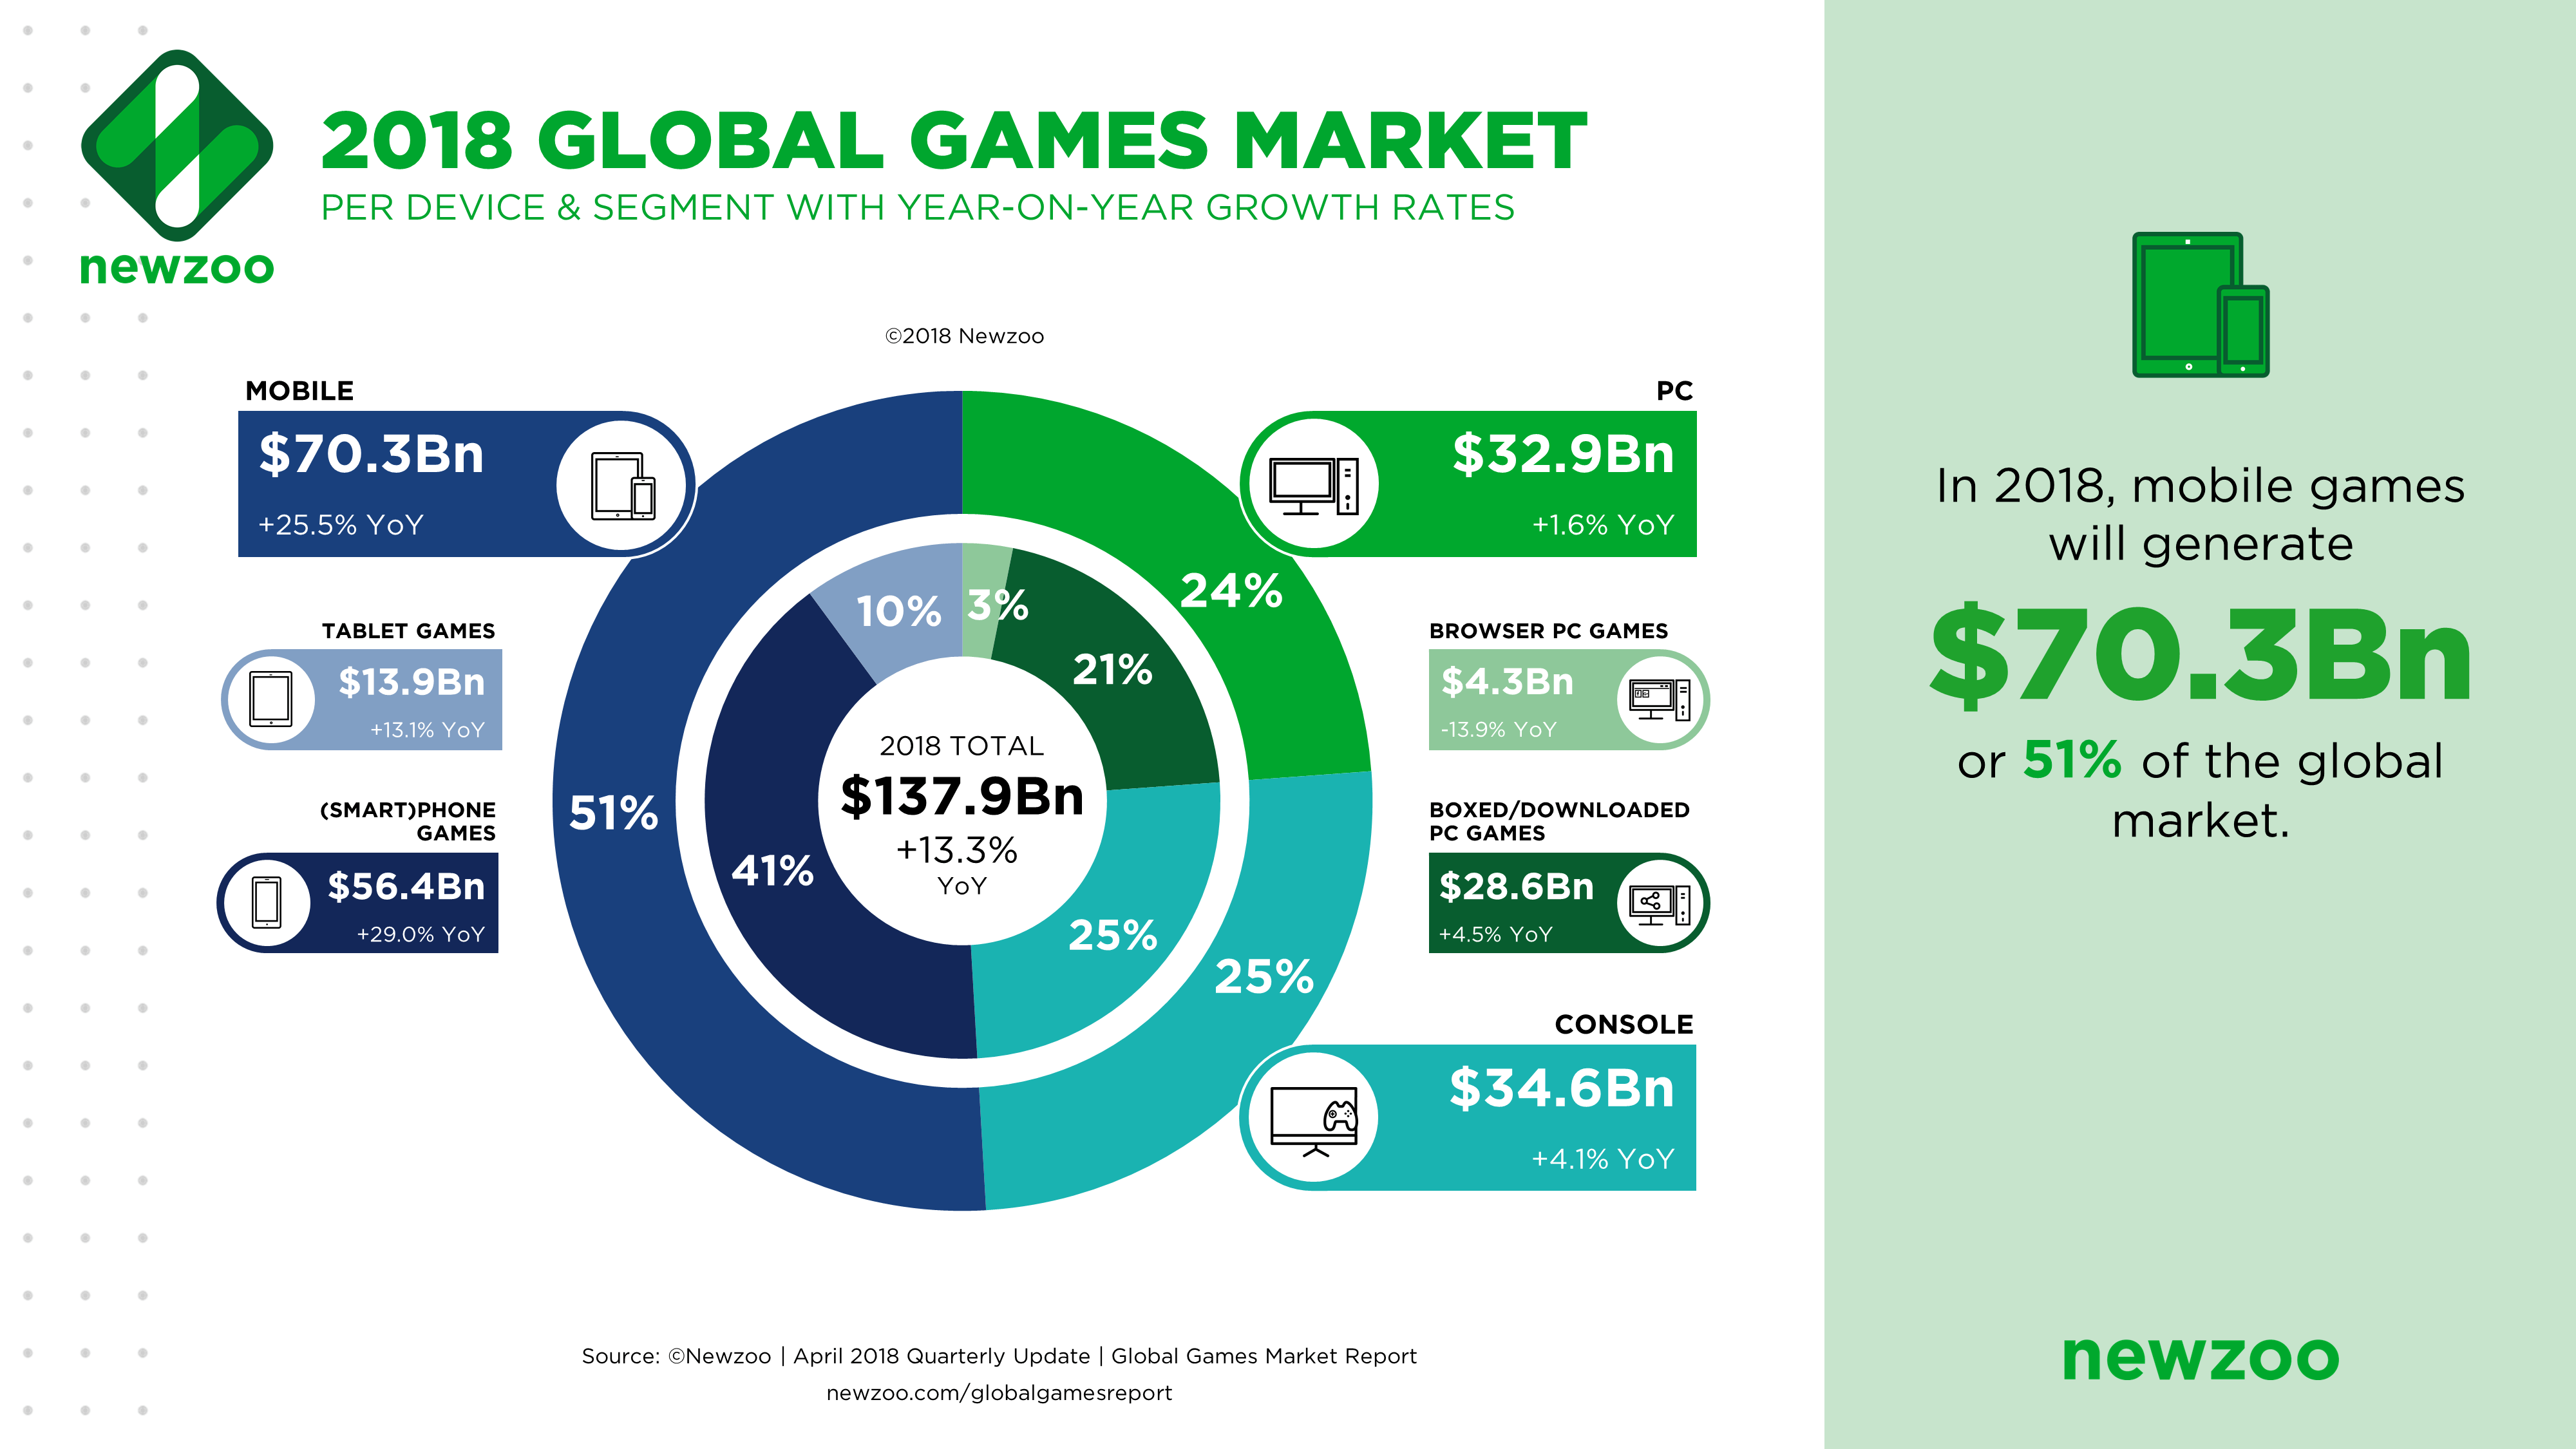
\includegraphics[width=0.5\textwidth]{02Antecedentes/contribucionesR/imagenes/merglo}
\end{figure}

Por primera vez, más de la mitad de todos los ingresos del juego provendrán del segmento móvil como vemos en la imagen{asdasd}. Los teléfonos inteligentes representarán el 80\% de esto, o \$ 56.4 mil millones, con el 20\% restante proveniente de tabletas.

\subsubsection{Salarios}
Para realizar un videojuego se necesita de diferentes profesiones para llevarlo a cabo.
En el siguiente cuadro \ref{tab:tablacostos} se mostrará la profesion y salario a recibir en la industria del videojuego en una empresa ya establecida al año 2014 segun la encuesta con una relación definida en experiencia.

% Please add the following required packages to your document preamble:
% \usepackage{multirow}
\begin{table}[htbp]
	\centering
\caption{Tabla de salarios dados en una empresa formal de videojuegos}
\label{tab:tablacostos}
\resizebox*{\linewidth}{!}{
	\begin{tabular}{|l|l|l|l|l|}
		\hline
		\textbf{Rama}                                                        & \textbf{Profesión}          & \textbf{Salario con -3años de exp.} & \textbf{Salario con 3-6años de exp.} & \textbf{Salario con +6años de exp.} \\ \hline
		\multirow{3}{*}{\textbf{Programadores e ingenieros}}                 & Programador                 & \$71,855 USD                        & \$79,877 USD                         & \$103,789 USD                       \\ \cline{2-5} 
		& Programador principal       &                                     & \$94,877 USD                         & \$116,151 USD                       \\ \cline{2-5} 
		& Director técnico            &                                     &                                      & \$135,781 USD                       \\ \hline
		\multirow{3}{*}{\textbf{Artistas y animadores}}                      & Animador                    & \$50,000 USD                        & \$55,547USD                          & \$82,230 USD                        \\ \cline{2-5} 
		& Artista principal           &                                     & \$71,029 USD                         & \$71,87576 USD                      \\ \cline{2-5} 
		& Director de arte            &                                     &                                      & \$110,000 USD                       \\ \hline
		\multicolumn{1}{|c|}{\multirow{2}{*}{\textbf{Diseñadores de juego}}} & Diseñador de juego          & \$53,000 USD                        & \$65,516 USD                         & \$77,768 USD                        \\ \cline{2-5} 
		\multicolumn{1}{|c|}{}                                               & Director creativo           &                                     & \$68,654 USD                         & \$101,944 USD                       \\ \hline
		\multicolumn{1}{|c|}{\multirow{3}{*}{\textbf{Productores}}}          & Productor asociado          &                                     & \$59,079 USD                         & \$61,912 USD                        \\ \cline{2-5} 
		\multicolumn{1}{|c|}{}                                               & Lider de proyecto           &                                     & \$73,500 USD                         & \$93,160 USD                        \\ \cline{2-5} 
		\multicolumn{1}{|c|}{}                                               & Productor ejecutivo         &                                     &                                      & \$126,833 USD                       \\ \hline
		\textbf{Profesional de audio}                                        & Director de sonido          &                                     &                                      & \$109,500 USD                       \\ \hline
		\multicolumn{1}{|c|}{\multirow{2}{*}{\textbf{Testers}}}              & Tester                      &                                     & \$38,833 USD                         &                                     \\ \cline{2-5} 
		\multicolumn{1}{|c|}{}                                               & Lider de control de calidad &                                     & \$60,417 USD                         & \$65,500 USD                        \\ \hline
		\multirow{3}{*}{\textbf{Negocios y administración}}                  & Marketing                   &                                     & \$73,500 USD                         &                                     \\ \cline{2-5} 
		& CEO                         &                                     &                                      & \$135,735 USD                       \\ \cline{2-5} 
		& Gerente ejecutivo           &                                     &                                      & \$156,731 USD                       \\ \hline
	\end{tabular}
}
\end{table}

\subsubsection{Presentación al cliente}
Un videojuego como cualquier software al momento de ser vendido al cliente puede encontrarse en dos presentaciones, una versión física o solo digital. En la siguiente tabla \ref{fiDi} se muestran las diferencias más destacables dadas por experiencia empresarial en el desarrollo por Velneo \cite{velneo2015}.

\begin{table}[htbp]
	\centering
	\caption{Tabla comparativa de un producto físico o digital por Velneo \cite{velneo2015}}
	\label{fiDi}
	\resizebox*{\linewidth}{!}{
\begin{tabular}{|l|l|l|}
	\hline
	\textbf{}                                             & \multicolumn{1}{c|}{\textbf{Físico}} & \multicolumn{1}{c|}{\textbf{Digital}} \\ \hline
	Coste de desarrollo                                   & sí                                   & sí                                    \\ \hline
	Coste de producción                                   & sí                                   & no                                    \\ \hline
	Coste de envío                                        & sí                                   & no                                    \\ \hline
	Riesgo de sobra/infra producir inventario             & sí                                   & no                                    \\ \hline
	Facturación por unidad vendida                        & mucho mayor                          & mucho menor                           \\ \hline
	Unidad vendida costea soporte                         & generalmente sí                      & imposible                             \\ \hline
	Porcentaje del precio de venta que percibe la empresa & 30\%-40\%                            & 70\%                                  \\ \hline
	Tiempo de cobro                                       & 90 días o más                        & 30 días                               \\ \hline
	Capacidad de llegar al público con marketing          & caro                                 & difícil                               \\ \hline
\end{tabular}
}
\end{table}

Aún así cabe mencionar que este es un aspecto general que involucra a cualquier software.

\subsubsection{Formas de ingreso}
Dentro de los videojuegos existen modelos de negocio que han dio cambiando a lo largo de los años y muchas de las veces depende del tipo del juego. Pero podemos definir las siguientes conforme lo visto y consumido en los últimos 5 años a la fecha del proyecto a presentar y con el apoyo de un artículo de la fundación UADE \cite{fundaciónuade2014} en la tabla \ref{tablaMoneVJ}.

\begin{table}[htbp]
	\centering
	\caption{Tabla comparativa de ventajas y desventajas de modelos de negocios de videojuegos de autoría propia}
	\label{tablaMoneVJ}
	\resizebox*{\linewidth}{!}{
	\begin{tabular}{llll}
		Nombre       & Descripción                                                                                                               & Ventaja                                                                                                                                                                                                                                                                                                                  & Desventaja                                                                                                                                                                                                                                                                                                                                                                            \\
		Pay-to-play  & Se debe pagar contenido y uso del videojuego                                                                              & \begin{tabular}[c]{@{}l@{}}* Rápido retorno de inversión\\ \\ * Sin limitación de juego\\ \\ * Puede re-dirigirse a otro modelo en caso de fracaso \\ \\ * Puede ser un producto físico, por lo que puede cobrarse contenido extra\\ \\ * Complementa con compras in-game\end{tabular}                                   & \begin{tabular}[c]{@{}l@{}}* No compras por desconocimiento del juego (más en móviles)\\ \\ * Inversión grande por enfoque a consolas \\ \\ * Jugadores esperan contenido de entretenimiento de larga duración y calidad\\ \\ * No hay soporte o cambios en el juego\\ \\ * Si es un producto físico debe costearse la producción\\ \\ * Necesita publicidad\end{tabular}             \\
		Free-to-play & Ofrece gratis contenido y uso del videojuego en su totalidad, se monetiza con publicidad y compras in-game                & \begin{tabular}[c]{@{}l@{}}* Contacto con los jugadores más rápido\\ \\ * Preferente para móviles\\ \\ * Preferente para juegos de poca inversión (que quiera escalar)\\ \\ * Complementa con compras in-game\end{tabular}                                                                                               & \begin{tabular}[c]{@{}l@{}}* Depende de la cantidad de jugadores activos\\ \\ * Debe ser un juego con adicción para sustentarse\\ \\ * Debe ser un juego “infinito”\\ \\ * Requiere continuas actualizaciones si desea mantenerse\\ \\ * Debe darse al jugador contenido nuevo a jugar\end{tabular}                                                                                   \\
		Freemium     & Ofrece gratis el uso del videojuego pero no se accede a todo su contenido, establece jerarquización de tipos de jugadores & \begin{tabular}[c]{@{}l@{}}* Conveniente para demos (versión lite)\\ \\ * Oportunidad de dar a conocer el juego\\ \\ * Oportunidad de convencimiento al jugador\\ \\ * Contacto con los jugadores más rápido\\ \\ * Preferente para móviles\\ \\ * Viable aun sí existen pocos jugadores dispuestos a pagar\end{tabular} & \begin{tabular}[c]{@{}l@{}}* Debe crearse contenido de calidad por pago\\ \\ * Debe existir un control y registro de jugadores para su jerarquización\\ \\ * Usualmente el contenido extra debe ser descargado de internet (por lo que implicaría otros gastos y recursos)\\ \\ * Recomendable ser un juego “infinito”\\ \\ * A veces requiere continuas actualizaciones\end{tabular} \\
		Suscripción  & Se debe pagar el contenido y uso del videojuego pero con limitaciones.                                                    & \begin{tabular}[c]{@{}l@{}}* Es combinable con otros modelos como el freemium\\ \\ * Permite a los jugadores explorar el juego completo por cierto tiempo\\ \\ * Oportunidad de dar a conocer el juego\end{tabular}                                                                                                      & \begin{tabular}[c]{@{}l@{}}* Debe crearse contenido de calidad por pago\\ \\ * Recomendable ser un juego “infinito”\\ \\ * A veces requiere continuas actualizaciones\\ \\ * Debe darse al jugador contenido nuevo a jugar\\ \\ * Depende de la cantidad de jugadores activos\\ \\ * Debe ser un juego con adicción para sustentarse\end{tabular}         
	                           
	\end{tabular}
}
\end{table}



\subsubsection{Ingredientes de monetización}
Los modelos de negocio anteriores pueden ser combinables con otros "ingredientes" de monetización para acrecentarlos ingresos. 
\begin{itemize}
	\item Dinero virtual: Es el medio de intercambio que utiliza un videojuego para poder formalizar las compras dentro de él. A menudo se suele diferenciar el virtual currency (dinero virtual que se consigue por las propias mecánicas del juego y con abundancia) y el hard currency (dinero virtual premium que se consigue con dinero real o con acciones muy concretas y con mucha escasez).
	\item Bienes virtuales: Son objetos intangibles que son comprados e intercambiados que sólo tienen sentido dentro del juego, muchas veces estos son comprados con dinero virtual. 
	\item Publicidad y patrocinio: Anuncios o productos presentados en el juego para darse a conocer.
	\item Bonificaciones y servicios virtuales: Son aceleradores de juego o servicios que mejoran el desempeño o facilitan en el juego.
	\item DLC (downloadable content): Es un contenido de descarga digital exclusivo y adicional de un videojuego que se vende por separado y posterior al lanzamiento de este. Suele lanzarse para alargar la longevidad del videojuego y para aprovechar su éxito comercial. Su adquisición no tiene sentido sin tener antes el videojuego ya que es un producto complementario y dependiente a él.
\end{itemize}
